% 
% Annual Cognitive Science Conference
% Sample LaTeX Paper -- Proceedings Format
% 

% Original : Ashwin Ram (ashwin@cc.gatech.edu)       04/01/1994
% Modified : Johanna Moore (jmoore@cs.pitt.edu)      03/17/1995
% Modified : David Noelle (noelle@ucsd.edu)          03/15/1996
% Modified : Pat Langley (langley@cs.stanford.edu)   01/26/1997
% Latex2e corrections by Ramin Charles Nakisa        01/28/1997 
% Modified : Tina Eliassi-Rad (eliassi@cs.wisc.edu)  01/31/1998
% Modified : Trisha Yannuzzi (trisha@ircs.upenn.edu) 12/28/1999 (in process)
% Modified : Mary Ellen Foster (M.E.Foster@ed.ac.uk) 12/11/2000
% Modified : Ken Forbus                              01/23/2004
% Modified : Eli M. Silk (esilk@pitt.edu)            05/24/2005
% Modified : Niels Taatgen (taatgen@cmu.edu)         10/24/2006
% Modified : David Noelle (dnoelle@ucmerced.edu)     11/19/2014

%% Change "letterpaper" in the following line to "a4paper" if you must.

\documentclass[10pt,letterpaper]{article}

\usepackage{cogsci}
\usepackage{pslatex}
\usepackage{apacite}
\usepackage{graphicx}

\title{Morphosyntactic and Referential Cues to the Identification of Generic Statements}
 
\author{{\large \bf Phil Crone} \\
	\texttt{pcrone@stanford.edu}\\
  Department of Linguistics \\
  Stanford University
  \And {\large \bf Michael C. Frank} \\
  \texttt{mcfrank@stanford.edu}\\
  Department of Psychology \\
  Stanford University}


\begin{document}

\maketitle


\begin{abstract}
Generic sentences (e.g. ``Birds fly.'') express generalizations about kinds, as opposed to non-generic sentences that are about specific individuals or groups of individuals (e.g. ``All birds fly.''). We investigate how language users use morphosyntactic and pragmatic cues to determine whether naturalistic sentences should receive generic interpretations. Experiment 1 demonstrates the effect of morphosyntactic features of a sentence's subject noun phrase (NP) on generic interpretation. Experiments 2 and 3 reveal that when a sentence's subject NP does not have an obvious reference in context, the sentence is more likely to receive a generic interpretation. 

\textbf{Keywords:} pragmatics; generics
\end{abstract}


\section{Introduction}

Generic sentences differ from non-generic sentences in that they express generalizations about kinds rather than properties of specific individuals or sets of individuals. For example, the sentence ``Birds fly'' express a general property of the kind \textit{bird}, whereas the sentence ``All birds fly'' states that for every member \textit{x} of the set consisting of all birds, \textit{x} flies. A key difference between generic and non-generic statements is that generics allow for exceptions. ``Birds fly'' is true despite the fact that some birds do not fly. ``All birds fly'' is false in virtue of the fact that there are individuals that are birds and do not fly \cite{Prasada:2000}. 

We can identify two distinct puzzles that generics pose for the study of natural language semantics and pragmatics. The first is how to provide adequate truth conditions for generic sentences. These truth conditions must account for the fact that generics allow for exceptions and other peculiarities, such as the fact that generics may be judged true even when the generalization does not hold for most members of the kind. A second puzzle is how language users solve the problem of identifying whether a sentence should receive a generic or non-generic interpretation; this problem arises because sentences are often ambiguous between generic and non-generic interpretations. The current study is concerned with the second puzzle.

Individuals use three types of cues to guide their interpretation of sentences as generic or non-generic: morphosyntactic features, pragmatic cues, and world knowledge \cite{Cimpian:2008, Cimpian:2011,Gelman:2003}. In English, the subject NP of a generic sentence is often a bare plural (``Birds fly.''), but indefinite singular (``A bird has wings.'') and definite singular (``The bird is a warm-blooded animal.'') NPs can also serve as subjects of generic sentences. Definite plural NPs (``The birds have feathers.'') are generally thought to force non-generic interpretations. Tense and aspect also cue whether it is to be interpreted generically. Generic sentences tend to use the simple present tense (``Birds fly.''), as opposed to the present progressive (``Birds are flying overhead.''), past tense (``Birds flew past my window.''), or tense/aspect categories \cite{Carlson:1977,Krifka:1995,Lyons:1977}.

In addition to these morphosyntactic cues, the preceding discourse and nonlinguistic factors may influence whether a sentence is interpreted as generic or non-generic. For example, if a unique bird is present in the context of an utterance of a sentence with the subject NP ``the bird,'' a non-generic interpretation in which this NP refers to the bird in context may be more likely. Conversely, if no such bird exists in the context, a generic interpretation may be preferred. Finally, world knowledge about the properties shared by members of a kind will influence the interpretation of potentially generic sentences. The sentence ``A bird does not fly'' is interpreted as a non-generic sentence about some particular bird (e.g. a penguin), given world knowledge that, in general, birds fly. 

Previous experimental work has demonstrated the relevance of these three factors to the identification of generic sentences. \citeA{Gelman:2003} show that adults and children as young as 3 show a preference for interpreting bare plurals as generic, as compared to definite plurals, and are more likely to interpret sentences as generic when the subject NP has no available referent in context. \citeA{Cimpian:2008} demonstrate that by age 3 children are less likely to assign a generic interpretation to a sentence when its subject NP has a possible referent in the preceding linguistic context. In addition, they show that children as young as 3 use knowledge about whether properties are generalizable to kinds as evidence about whether to interpret sentences as generic or not. Finally, \citeA{Cimpian:2011} show that 3-year-olds use definiteness of subject NPs as a cue to identifying generics and that adults and children as young as 4 use tense and aspect to identify generics.

The present study differs from previous work in several respects. The majority of previous work on the identification of generics has focused on children's abilities, whereas the current study is primarily concerned with how adults identify generics. The focus on children's identification of generics stems in part from the fact that children face an inductive problem not faced by adult language users regarding which types of NPs refer to kinds. However, recent work emphasizing the probabilistic nature of language comprehension \cite{Frank:2012,Levy:2008} suggests that adults face a similar problem. On this view, language users resolve uncertainty in language comprehension via probabilistic inference to the most likely interpretation. In the specific case of identifying generics, we can view adults as reasoning about the likelihood of an utterance being generic given morphosyntactic features of the sentence, features of the context, and the listeners' world knowledge. 

The current study also differs from previous work by collecting naturalistic examples of generic and non-generic sentences generated by study participants. This approach allows for a more realistic representation of how genericity is used in natural language. The approach also allows for consideration of examples that are more ambiguous between generic and non-generic interpretations than examples created by experimenters. 

\section{Experiment 1: Morphosyntactic Cues}

As discussed above, the number and definiteness of a sentence's subject NP influence its interpretation as generic or non-generic \cite{Carlson:1977,Krifka:1995,Lyons:1977}. Previous work investigating morphosyntactic cues to genericity have fixed the number of the subject NP as either singular \cite{Cimpian:2011} or plural \cite{Gelman:2003} and only manipulated definiteness. In Experiment 1, we considered number, definiteness, and their interaction, on the interpretation of generics. We asked participants to perform a sentence completion task in which the subject NP was provided. Participants were then asked to indicate whether the sentences they produced were about specific individuals or kinds.

\subsection{Method}

\subsubsection{Participants} \quad We recruited 100 participants to participate through Amazon's Mechanical Turk website. Participants were restricted to individuals within the United States and were paid 50 cents to complete the study. The study took approximately 14 minutes to complete.

\subsubsection{Stimuli} \quad Forty-eight nouns were chosen to use as the bases for subject NPs. To ensure diversity among these subject NPs, twenty-four nouns were animate and twenty-four were inanimate. For each study participant, a random set of twelve nouns were assigned morphosyntactic features using a \(2 \times 2\) factorial design crossing number (singular, plural) with definiteness (definite, indefinite). Exactly half of nouns assigned to each factorial point were animate and half were inanimate. Base nouns were then programmatically edited to reflect the assigned number and definiteness values and create full NPs. For example, if the noun ``panda'' were assigned values \textit{plural} and \textit{definite}, the full NP would be ``the pandas.''

In the first part of the experiment, participants saw a single NP followed by a single-line text box. They were instructed to ``write a sentence starting with the phrase below.'' In the second part of the experiment, participants were shown the sentences they had written in the first part of the experiment. They were shown one sentence at a time and asked whether the sentence was about a specific \textit{noun} (for singular NPs), a specific group of \textit{nouns} (for plural NPs), or about \textit{nouns} in general. Participants indicated their response using a 5-point Likert scale with the following values: ``Definitely about a specific \textit{noun}/group of \textit{nouns} (=1),'' ``Probably about a specific \textit{noun}/group of \textit{nouns},'' ``Not sure,'' ``Probably about \textit{nouns} in general,'' ``Definitely about \textit{nouns} in general (=5).''

\subsubsection{Procedure} \quad We first presented participants with four example noun phrases. After these first four items, participants were shown an example sentence that they could have used for the example noun phrase. These sentences were constructed to favor non-generic interpretations for all NP types. After seeing the examples, participants were informed that they would not receive any feedback for the rest of the experiment.

Participants then began the first part of the experiment. All forty-eight subject NPs were presented in pseudorandom order counterbalanced so that no two consecutive NPs matched in both number and definiteness. We required participants to provide a sentence completion for each item and required that sentence completions be a minimum of six characters long. After completing part one, participants were told that they were entering the second part of the experiment and were informed that they would be evaluating sentences' genericity. They then evaluated the sentences they had produced in part one in the manner described above. Once again, sentences were presented in a pseudorandom order counterbalanced so that no two consecutive NPs matched in both number and definiteness. After judging all forty-eight sentences, they were then required to provide their native language. We measured reaction times for each item, measured from the time the item was presented until the time a response was submitted. 

\subsubsection{Data Analysis} \quad We excluded 4 participants for indicating that their native language was not English. Thus, responses from 96 participants were analyzed. In addition, responses from items whose reaction times were greater than 2 standard deviations from the mean for the second part of the experiment.

\begin{table*}
\begin{center} 
\caption{Example Productions from Experiment 1. Generic sentences received ratings of 5; non-generics received ratings of 1.} 
\label{sample-table} 
\vskip 0.12in
\begin{tabular}{cccc} 
\hline
Definiteness    &  Number & Genericity & Examples \\
\hline
Indefinite        &   Singular & Generic & ``A cow eats grass.'', ``A bicycle is a convenient form of transportation.''\\
Indefinite  &   Singular & Non-generic & ``A dog is sleeping on the porch.'', ``A light bulb was dropped and exploded.''\\
Indefinite           &   Plural & Generic & ``Gorillas are primates.'', ``Towels are useful after showering.''\\
Indefinite         &   Plural  & Non-generic & ``Cats are circling the fishtank.'', ``Kites were flying at the beach.''\\
Definite        &   Singular & Generic & ``The camel uses his humps to conserve water.'', ``The clock tells time.''  \\
Definite  &   Singular & Non-generic & ``The bear is moving closer to us.'', ``The bed is unmade.''\\
Definite           &   Plural & Generic & ``The kangaroos carry babies in pouches.'', ``The trumpets are loud.'' \\
Definite         &   Plural & Non-generic & ``The rabbits are digging holes in the yard.'', ``The couches were dusty and old.''\\
\hline
\end{tabular} 
\end{center} 
\end{table*}

\subsection{Results \& Discussion}

Paragraph about figure.

To analyze these findings, we fit a linear mixed-effects model to predict participants' ratings of their sentences for genericity. We examined the interaction between animacy, definiteness, and number of subject NPs.\footnote{All mixed-effects models were fit using the lme4 package in R version 3.1.2. The model specification was as follows: \texttt{response} \(\sim\) \texttt{animacy * definiteness * number + (animacy + definiteness + number | WorkerId) + (definiteness + number | subject)}. For each effect, \(p\) values were calculated by treating the \(t\) statistic as if it were a \(z\) statistic \cite{Barr:2013}.} The model shows main effects of animacy, definiteness, and number. Sentences with indefinite NP subjects were rated significantly more generic (\(\beta = 1.745, t = 14.169, p < 0.001\)). Sentences with singular NP subjects (\(\beta = -0.302, t = -3.450, p < 0.001\)), and inanimate subjects (\(\beta = -0.503, t = -5.732, p < 0.001\)), were rated less generic. In addition, the model revealed an interaction effect between definiteness and number such that indefinite singulars were rated significantly less generic (\(\beta = -1.023, t = -9.913, p < 0.001\)). Finally, there was a significant three-way interaction such that inanimate, indefinite singulars were rated significantly more generic (\(\beta = 0.536, t = 3.669, p < 0.001\)). 

The results are consistent with previous findings that indefinite singulars and bare plurals facilitate generic interpretations compared to definite singulars and definite plurals, respectively \cite{Cimpian:2011, Gelman:2003}. However, these results also show that plurality is independently associated with genericity, which has not been previously acknowledged. The interaction between definiteness and plurality reveals a superadditive effect by which indefinite singulars support generic interpretation less than bare plurals. This is unsurprising, as bare plurals are often taken to be the canonical subject type for English generics \cite{Carlson:1977,Krifka:1995,Lyons:1977}. The effect of animacy on genericity ratings is consistent with previous findings that both children and adults produce more generic statements in describing animals than in describing artifacts \cite{Brandone:2009}.

The most unexpected finding is the fact that definite plurals were found to be more generic overall than definite singulars, despite the general view that definite singulars, but not definite plurals, allow for generic interpretations in English. This result had us consider whether our methodology measured some property other than genericity. However, inspection of definite plurals that received high genericity ratings suggested that these ratings were appropriate (Table 1).

This experiment demonstrated the role of morphosyntactic and, in the case of animacy, world knowledge cues to identifying generic statements. However, this experiment left contextual cues unaddressed. We therefore conducted two more experiments to examine the role that context plays in identifying generics. 

\section{Experiment 2A: Contextual Cues in Production}

Experiment 2A investigated the role of context as a cue to identifying generics. Specifically, this experiment examined whether language users will be less likely to treat a subject NP as generic when it has a possible referent in the context.

\subsection{Method}

\subsubsection{Participants} \quad We recruited 100 participants to participate through Amazon's Mechanical Turk website. Participants were restricted to individuals within the United States and were paid 50 cents to complete the study. The study took approximately 14 minutes to complete.

\subsubsection{Stimuli} \quad The stimuli were almost identical to those used in Experiment 1. However, in part 1 of the experiment, each subject NP was accompanied by an image depicting either one or five instances of the animal or artifact denoted by the subject NP (Figure 1). Images with only one instance of the animal or artifact were taken directly from the Bank of Standardized Stimuli version 2.0 \cite{Brodeur:2014}. Images with multiple instances of the animal or artifact were created from the single instance images using Pixelmator version 3.2.1. The number of individuals in the image either matched or mismatched the number of the subject NP. Half of items for each subject NP type were paired with matching images and half were paired with mismatching images. Participants were instructed to describe the image in their sentence completion. The images only appeared for the sentence completion portion of the experiment; they did not appear 

\subsubsection{Procedure} \quad The procedure was the same as that in Experiment 1. For the four example items, two items were randomly chosen to have matching images, the other items had mismatching images. As in Experiment 1, the order of items in both parts of the experiment were pseudorandomized with counterbalancing to ensure that no two consecutive items used subject NPs with the same number and definiteness features. The order of images was not controlled.

\subsubsection{Data Analysis} \quad We excluded 2 participants for indicating that their native language was not English. Thus, responses from 98 participants were analyzed. In addition, responses from items whose reaction times were greater than 2 standard deviations from the mean for the second part of the experiment.

\begin{figure}[t]
\begin{center}
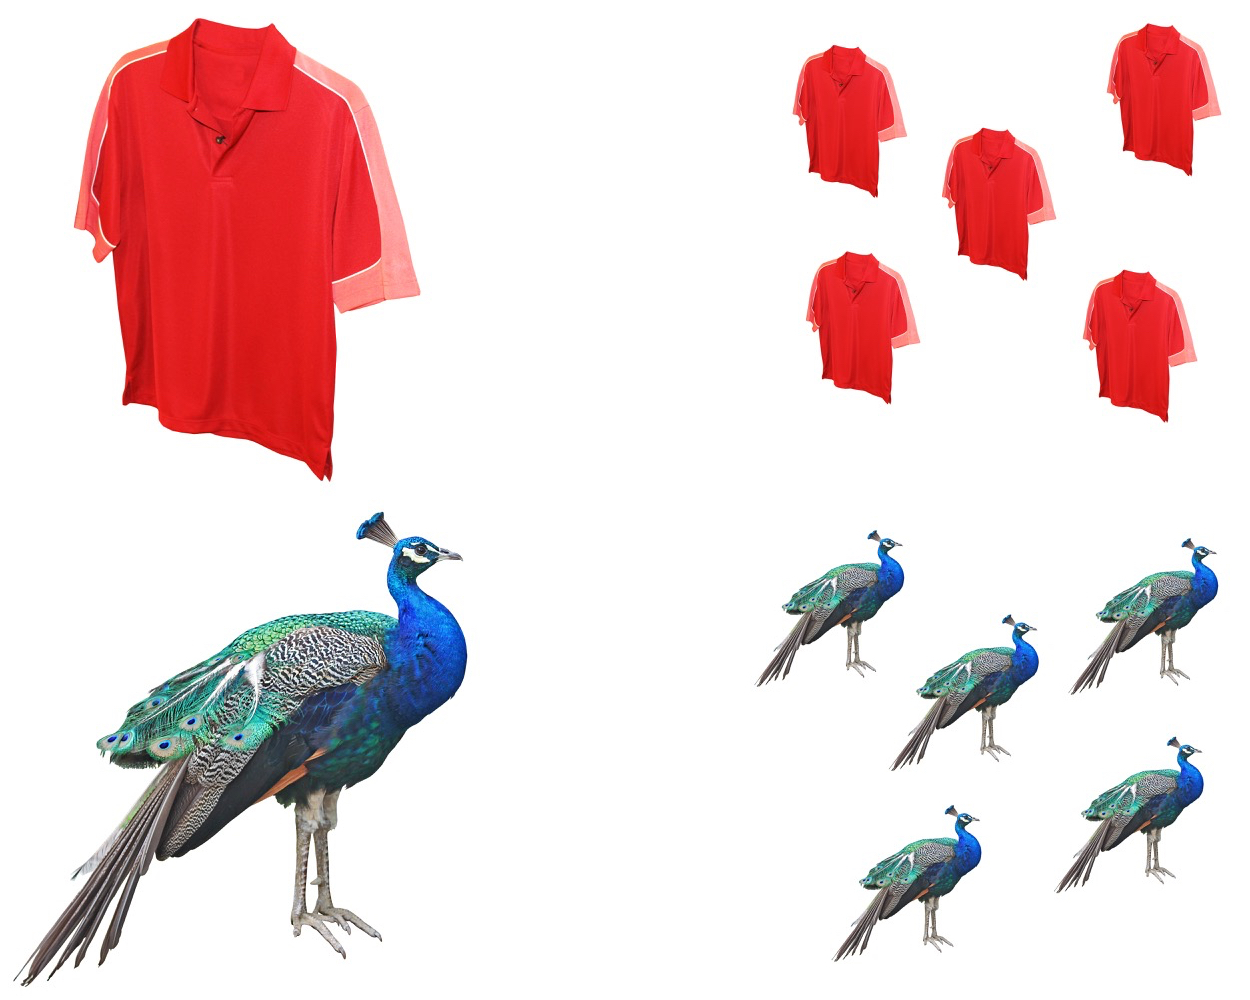
\includegraphics[width=0.35\textwidth]{stimuli.jpg}
\end{center}
\caption{Examples of images used in Experiments 2A, 2B, and 3. Clockwise from upper left: single shirt, multiple shirts, multiple peacocks, single peacock.} 
\label{sample-figure}
\end{figure}

\subsection{Results \& Discussion}

Paragraph about figure.

As in Experiment 1, we fit a linear mixed-effects model to predict participants' genericity ratings of their sentences. We examined the interaction of animacy, definiteness, and number of the subject NP, as well as image match/mismatch.\footnote{The model specification was as follows: \texttt{response} \(\sim\) \texttt{animacy * definiteness * number * image + (animacy + definiteness + number + image | WorkerId) + (definiteness + number + image | subject)}.} The model revealed significant main effects of animacy, definiteness, and image. Sentences with indefinite subject NPs were rated more generic (\(\beta = 1.023, t = 7.518, p < 0.001\)), while sentences with inanimate subjects were rated less generic (\(\beta = -0.742, t = -4.005, p < 0.001\)). Sentences produced with an image that did not match the subject NP in number were also rated significantly more generic (\(\beta = 0.389, t = 3.414, p < 0.001\)). The model also revealed interaction effects between definiteness and number such that sentences with indefinite singular subjects were significantly less generic (\(\beta = -0.340, t= -2.170, p < 0.05\)), and between definiteness and image such that sentences with indefinite subjects that appears with mismatching images were less generic (\(\beta = -0.426, t = -2.731, p < 0.001\)). Finally, the model showed a significant three-way interaction such that inanimate, indefinite subjects with mismatching images were rated significantly more generic (\(\beta = 0.567, t = 2.571, p < 0.05\)).

Several of these effects are similar to those observed in Experiment 1, and can be interpreted similarly. The main effect of subject NP number that was observed in Experiment 1 did not appear in the model for Experiment 2; the effect of number in the model was in the expected direction, with sentences with singular subjects being rated less generic, but was not significant (\(\beta = -0.162, t = -1.397, p > 0.1\)). The most important finding of Experiment 2A was the effect of image match/mismatch. Participants generated more generic sentences when the subject NP did not have a clear referent in the image. This results suggests that language users are sensitive to whether an NP refers in context in producing generics.

This result is similar to the finding of \citeA{Gelman:2003}, where it was shown that children and adults are more likely to interpret pronouns as generic when the only possible contextual referent mismatches in number. However, Gelman and Raman hypothesized that this effect would only be seen for plural pronouns in a context with only singular referents. The results of Experiment 2A suggest this is incorrect, due to the main effect of image mismatch and the lack of interaction effects between image and number. Generics are supported when NPs fail to have a reference in context, regardless of whether these NPs are singular or plural.

We note that this experiment focused on whether generic sentences are produced more often for a given NP when this NP has a contextual referent. However, this is a a slightly different question from that of whether listeners are more likely to interpret sentences as generic when the subject NP fails to refer in context. We investigated this question in Experiment 2B. 

\section{Experiment 2B: Contextual Cues in Comprehension}

\subsection{Method}

\subsubsection{Participants} \quad We recruited 100 participants to participate through Amazon's Mechanical Turk website. Participants were restricted to individuals within the United States and were paid 30 cents to complete the study. The study took approximately 4 minutes to complete.

\subsubsection{Stimuli} \quad Since this experiment focused on interpretation, there was no production portion of the experiment, as there was in Experiments 1 and 2A. Each participant in Experiment 2B was assigned some set of sentences produced by a participant in Experiment 2A. For everyThis set consisted of the twenty-four sentences a participant in Experiment 2A produced while viewing a picture that matched the subject NP in number. Each participant in Experiment 2A was matched with two individuals in Experiment 2B. In addition to the two non-native English speakers from Experiment 2A, three participants from Experiment 2A were not matched with participants in Experiment 2B because they had produced possibly offensive and inappropriate sentences.

The stimuli were presented in a manner similar to part two of Experiment 2A. However, images were displayed above each sentence. Half of the sentences for each NP subject type were presented with an image that matched the subject NP in number, while half were presented with an image that mismatched in number. For each item that was seen with a matching image by one participant, that item was seen with a mismatching image by a second participant. Participants were told that other Mechanical Turk workers had produced the sentences they were evaluating in order to describe the same pictures they were seeing.

\subsubsection{Procedure} \quad The procedure was the same as that for part 2 of Experiments 1 and 2A. Participants were instructed to pay attention to the images they saw and consider what the other Mechanical Turk worker was thinking when he/she produced each sentence. For the four example items, two items were randomly chosen to have matching images, the other items had mismatching images. Participants did not receive any feedback after providing genericity judgments for the four example items. As in Experiments 1 and 2A, the order of items in both parts of the experiment were pseudorandomized with counterbalancing to ensure that no two consecutive items used subject NPs with the same number and definiteness features. The order of images was not controlled.

\subsubsection{Data Analysis} \quad We excluded 5 participants for indicating that their native language was not English. Thus, responses from 185 participants were analyzed. In addition, responses from items whose reaction times were greater than 2 standard deviations from the mean for the second part of the experiment.

\subsection{Results \& Discussion}

Paragraph about figured

As in Experiment 2A, we fit a linear mixed-effects model to predict participants' genericity ratings from animacy, definiteness, number, and image match/mismatch, as well as the associated interactions.\footnote{The model specification was as follows: \texttt{response} \(\sim\) \texttt{animacy * definiteness * number * image + (animacy + definiteness + number + image | WorkerId) + (definiteness + number + image | subject)}.} The model revealed significant main effects of definiteness, number, and image. Sentences with indefinite subject NPs were rated more generic (\(\beta = 1.401, t = 11.718, p < 0.001\)), while sentences with singular subjects were rated less generic (\(\beta = -0.421, t = -3.642, p < 0.001\)). Sentences produced with an image that did not match the subject NP in number were also rated significantly more generic (\(\beta = 0.382, t = 3.604, p < 0.001\)). The model also revealed interaction effects between between definiteness and image such that sentences with indefinite subjects that appears with mismatching images were less generic (\(\beta = -0.426, t = -2.731, p < 0.001\)) and between animacy and image such that sentences with inanimate subjects and mismatching images were less generic (\(\beta = -0.380, t=-2.508, p<0.05\)). Finally, the model showed a significant three-way interaction such that inanimate, indefinite subjects with mismatching images were rated significantly more generic (\(\beta = 0.431, t = 2.028, p < 0.05\)).

The results again largely resemble those of Experiments 1 and 2A. As in Experiment 1, there was a significant effect of the number of the subject. However, unlike Experiments 1 and 2A, we found no significant main effect of animacy for \(p < 0.05\), although inanimates were rated as less generic than animates (\(\beta = -0.280, t = -1.822, p = 0.069\)). As in Experiment 2A, the main finding in Experiment 2B was the effect of the image either matching or mismatching the subject NP in number. We find that listeners are more likely to interpret a sentence as generic when its subject NP fails to refer in context. This effect is consistent across all NP types examined in the study.

\section{Experiment 3: Ambiguous Sentences}

\subsection{Method} 

\subsubsection{Participants} \quad

\subsubsection{Stimuli} \quad

\subsubsection{Procedure} \quad

\subsubsection{Data Analysis} \quad

\subsection{Results \& Discussion}


\section{General Discussion}


\section{Acknowledgments}

Place acknowledgments (including funding information) in a section at
the end of the paper.

\bibliographystyle{apacite}

\setlength{\bibleftmargin}{.125in}
\setlength{\bibindent}{-\bibleftmargin}

\bibliography{Generics}


\end{document}
